\begin{usecase}{Add Event Manually}
  \ucbasicinfo{High}{Regular}
  \ucshortdescription{This UC allows users to add events manually.}
  \uctrigger{The user clicks add event manually icon or a date on the calendar and adds the events.}
  \ucactors{User}{None}
  \ucpreconditions{The user is logged into the application.}
  \ucrelationships{N/A}{N/A}{N/A}
  \ucinputsoutputs{
    \begin{itemize}
      \item \textbf{Event Name} (Source: User)
      \item \textbf{Event Location} (Source: User)
      \item \textbf{Is all day?} (Source: User)
      \item \textbf{Event Date (Start and End)} (Source: User)
      \item \textbf{Event Time (Start and End)} (Source: User)
      \item \textbf{Note} (Source: User)
      \item \textbf{Notifications/Reminders} (Source: User)
    \end{itemize}
  }{
    \begin{itemize}
      \item \textbf{New Calendar event}
            (Destination: Calendar)
    \end{itemize}
  }
  \ucmainflow{
    \begin{enumerate}
      \item The user clicks the add event manually icon in the top corner `+'.
            \ucinfo{The add event manually form is displayed.}
      \item The user sets the details of the event in the respective fields and saves the event.
            \ucinfo{The event is displayed on the calendar with its details.}
    \end{enumerate}
  }
  \ucalternateflows{
    \begin{enumerate}
      \item If the validation fails the user can try again after fixing the issues.
    \end{enumerate}
  }
  \ucexceptions{
    \begin{itemize}
      \item The end time is before the start time.
      \item The user attempts to save the event without filling in mandatory fields.
    \end{itemize}
  }
  \ucconclusion{The UC ends when the event has been successfully added to the calendar, and displayed.}
  \ucpostconditions{The event is successfully added to the calendar and displayed in the correct time slot.}
  \ucspecialrequirements{The interface must be simple and allowing users to input events with less efforts.}
\end{usecase}

\begin{figure}[!h]
  \centering
  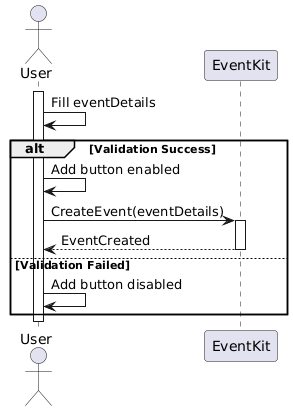
\includegraphics[width=\textwidth]{images/docs/diagrams/sequence-diagrams/all-sequence-diagrams/Add Event Manually.png}
  \caption{Add Event Manually Sequence Diagram}
  \label{fig:seq/add-event-manually}
\end{figure}

The ``Add Event Manually Sequence Diagram'' illustrates a simple flow of creating a calendar event. The sequence starts with the user filling in event details. The system then performs validation by EventKit:

\begin{enumerate}
  \item If validation succeeds:
        \begin{itemize}
          \item The Add button becomes enabled
          \item User can proceed to create the event
          \item EventKit processes the creation request
          \item Event creation confirmation is returned
        \end{itemize}
  \item If validation fails:
        \begin{itemize}
          \item The Add button remains disabled
          \item User must correct the input before proceeding
        \end{itemize}
\end{enumerate}

This straightforward workflow ensures data validation before any attempt to create an event, preventing invalid entries from being submitted to the calendar system.